\documentclass{article}
\usepackage[paperwidth=32cm,paperheight=18cm,margin=0.9cm]{geometry}
\usepackage{tikz}
\usetikzlibrary{arrows.meta}
\usepackage[T1]{fontenc}
\usepackage{helvet}
\renewcommand{\familydefault}{\sfdefault}
\pagestyle{empty}
\definecolor{ink}{HTML}{14202B}
\definecolor{teal}{HTML}{0C5F59}
\definecolor{paper}{HTML}{F4F1EA}
\definecolor{brown}{HTML}{5C4A3A}
\pagecolor{paper}

\tikzset{
  flowstep/.style={draw=ink, line width=1pt, rounded corners=3pt, align=left, fill=white, text width=13.2cm, inner sep=8pt, font=\large, minimum height=1.15cm}
}

\begin{document}
\begin{center}
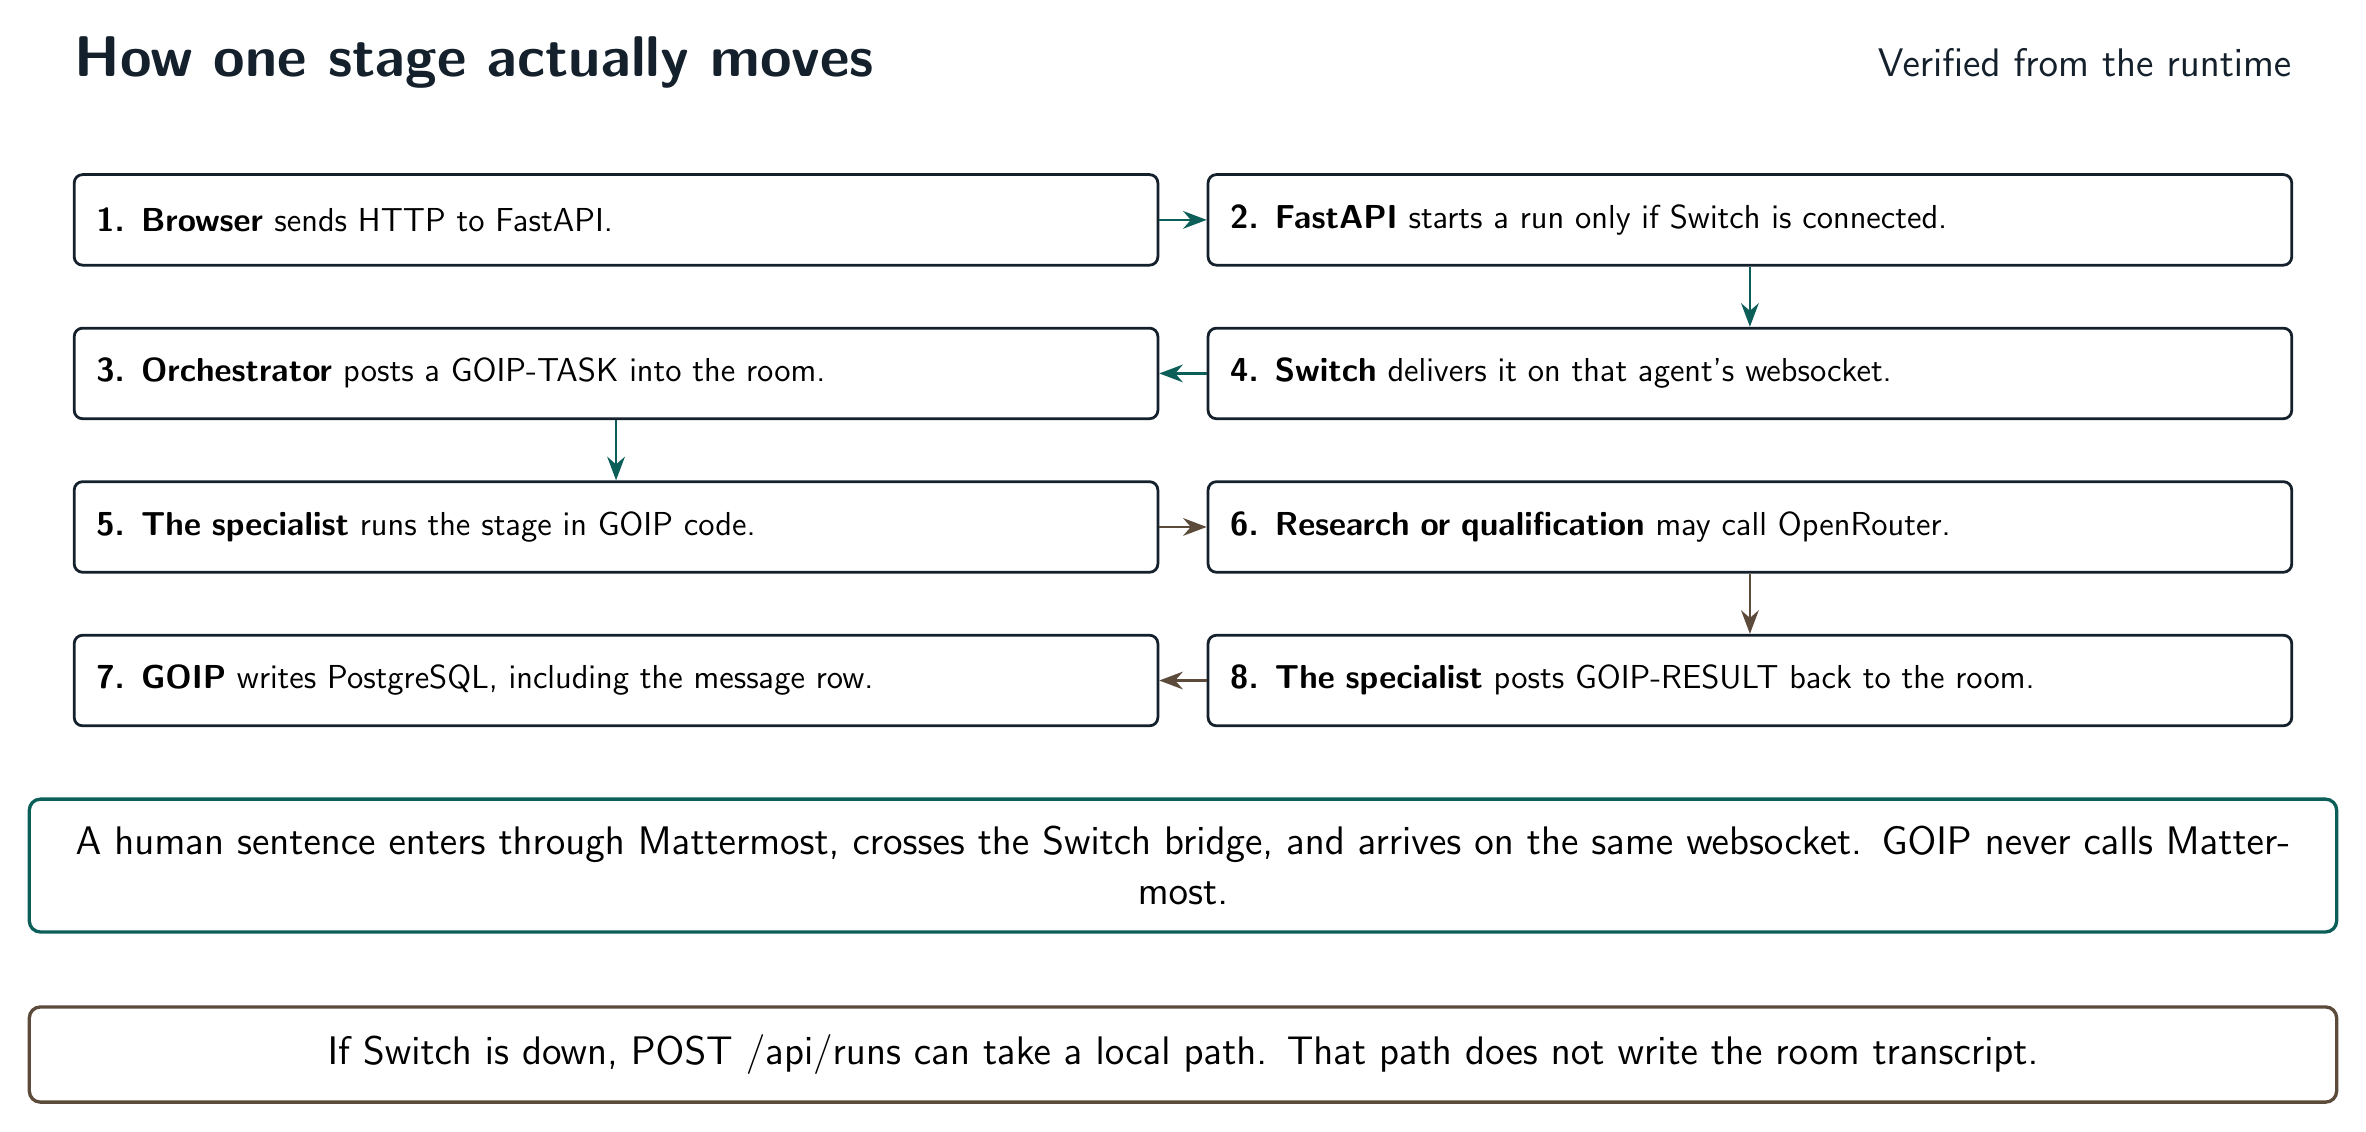
\begin{tikzpicture}
  \node[font=\huge\bfseries, text=ink, anchor=west] at (-14.2,7.5) {How one stage actually moves};
  \node[font=\Large, text=ink, anchor=east] at (14.2,7.5) {Verified from the runtime};

  \node[flowstep] (a) at (-7.2,5.5) {\textbf{1. Browser} sends HTTP to FastAPI.};
  \node[flowstep] (b) at (7.2,5.5) {\textbf{2. FastAPI} starts a run only if Switch is connected.};
  \node[flowstep] (c) at (-7.2,3.55) {\textbf{3. Orchestrator} posts a GOIP-TASK into the room.};
  \node[flowstep] (d) at (7.2,3.55) {\textbf{4. Switch} delivers it on that agent's websocket.};
  \node[flowstep] (e) at (-7.2,1.6) {\textbf{5. The specialist} runs the stage in GOIP code.};
  \node[flowstep] (f) at (7.2,1.6) {\textbf{6. Research or qualification} may call OpenRouter.};
  \node[flowstep] (g) at (-7.2,-0.35) {\textbf{7. GOIP} writes PostgreSQL, including the message row.};
  \node[flowstep] (h) at (7.2,-0.35) {\textbf{8. The specialist} posts GOIP-RESULT back to the room.};

  \node[draw=teal, line width=1.2pt, rounded corners=4pt, fill=white, text width=28.6cm, align=center, inner sep=10pt, font=\Large] at (0,-2.7)
  {A human sentence enters through Mattermost, crosses the Switch bridge, and arrives on the same websocket. GOIP never calls Mattermost.};

  \node[draw=brown, line width=1.2pt, rounded corners=4pt, fill=white, text width=28.6cm, align=center, inner sep=10pt, font=\Large] at (0,-5.1)
  {If Switch is down, POST /api/runs can take a local path. That path does not write the room transcript.};

  \draw[-{Stealth[length=3mm]}, teal, thick] (a.east) -- (b.west);
  \draw[-{Stealth[length=3mm]}, teal, thick] (b.south) -- (d.north);
  \draw[-{Stealth[length=3mm]}, teal, thick] (d.west) -- (c.east);
  \draw[-{Stealth[length=3mm]}, teal, thick] (c.south) -- (e.north);
  \draw[-{Stealth[length=3mm]}, brown, thick] (e.east) -- (f.west);
  \draw[-{Stealth[length=3mm]}, brown, thick] (f.south) -- (h.north);
  \draw[-{Stealth[length=3mm]}, brown, thick] (h.west) -- (g.east);
\end{tikzpicture}
\end{center}
\end{document}
